\documentclass[../../course]{subfiles}

\renewcommand\thesection{\arabic{section}}


\begin{document}

\def\freqXOne{28}
\def\freqXTwo{28.1}
\def\freqXThree{56}

\section{Generating Complex Sequences} \label{sec:wrkGenCompSeqs}

In section \ref{lst:threeSeqs} we generated three signals with three different
frequencies. The important thing to notice is that, they all are real valued
sequences. In this section, we will see how we can combine\footnote{as real and
imaginary part of a complex sequence} these signals into \emph{complex} sequences.

\subsection{Mixing of Signals}

We have three different distinct sequences, so how we can mix these signals into
more diverse \emph{complex} sequences ? This can be simply done by taking one of our
\emph{real valued} sequence as the \emph{real part} of the \emph{complex} sequence
and another \emph{real valued} sequence as the \emph{imaginary part} of the
\emph{complex} sequence. By doing so, one may encounter that there are many ways
to arrange these sequences. Or so to say, there are many different combinations\footnote{of
different real and imaginary sequences}, thus generating there many distinct \emph{complex}
sequences.


\begin{figure} [H]

    \centering

    \begin{tabularx} {\textwidth} {
            *{3}{>{\centering\arraybackslash}X}
        }

        & & \\

        \adjustbox{max width = 0.3\textwidth} {
            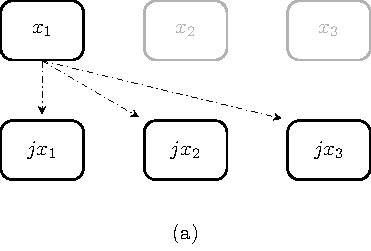
\includegraphics[height = 0.3\textheight] {tikzpics/epicCplxCombFirst.pdf}
        }

        &

        \adjustbox{max width = 0.3\textwidth} {
            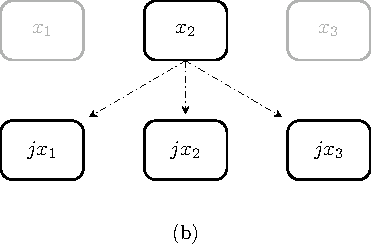
\includegraphics[height = 0.3\textheight] {tikzpics/epicCplxCombSecond.pdf}
        }

        &

        \adjustbox{max width = 0.3\textwidth} {
            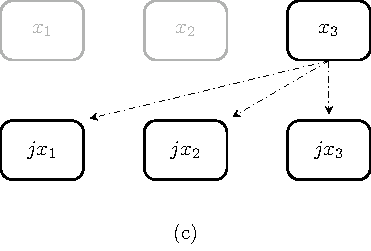
\includegraphics[height = 0.3\textheight] {tikzpics/epicCplxCombThird.pdf}
        }

        \\

        \captionof{figure} {
            Taking $x_{1}$ as real part and $x_{1}$, $x_{2}$, and $x_{3}$ as imaginary parts.
        }
        \label{fig:cplxCombFirst}

        &

        \captionof{figure} {
            Taking $x_{2}$ as real part and $x_{1}$, $x_{2}$, and $x_{3}$ as imaginary parts.
        }
        \label{fig:cplxCombSecond}

        &

        \captionof{figure} {
            Taking $x_{3}$ as real part and $x_{1}$, $x_{2}$, and $x_{3}$ as imaginary parts.
        }
        \label{fig:cplxCombThird}

    \end{tabularx}

\end{figure}

As we can see from figures \ref{fig:cplxCombFirst} to \ref{fig:cplxCombThird} there is a
total of $3 \times 3 = 9$ different ways to combine these three signals. In the upcoming
subsections we will see each of these combinations in detail. Table \ref{tbl:cplxSeqs}
shows the total list of \emph{complex} sequences we'll be generating.

Before that, let's use python to combine our \emph{real} sequences into \emph{complex}
sequences.

\subsection{Combining Sequences using Python}

%python/combine_sequences.py%
\begin{minted}[breaklines, autogobble, mathescape] {python}
    import numpy as np
    import pandas as pd

    F = 28
    t = np.linspace(0, 1.25 * np.pi / 4, 2500)

    x1 = np.sin( 2 * np.pi * F * t)
    x2 = np.sin( 2 * np.pi * (F + 0.1) * t)
    x3 = np.sin( 2 * np.pi * 2 * F * t)

    real = [x1, x2, x3]
    imag = [x1, x2, x3]

    pd.DataFrame( {
        "x1": x1[0:625],
        "x2": x2[0:625],
        "x3": x3[0:625],
    }).to_csv(
        "../data/short_sequences.csv", sep = " ", index_label = "time"
    )

    cplx_labels = [
        "complex_a",
        "complex_b",
        "complex_c",
        "complex_d",
        "complex_e",
        "complex_f",
        "complex_g",
        "complex_h",
        "complex_i",
    ]

    cplx = []

    for r in real:
        for i in imag:
            cplx.append(pd.DataFrame({
                "real": r,
                "imag": i,
            }))

    for i in range(len(cplx)):
        cplx[i].to_csv(
            "../data/" + cplx_labels[i] + ".csv", sep = " ", index_label = "time"
        )

\end{minted}


\begin{figure} [H]
    \centering

    %% \renewcommand{\arraystretch}{1.2}
    \begin{tabularx} {\textwidth} {
            *{1}{>{\centering\arraybackslash}X}
        }

        \\

        { \begin{tabularx} {\textwidth} {
                *{6}{>{\centering\arraybackslash}X}
            }

            \toprule
            \textsc{Combination Name} & \textsc{Complex Sequence} &
            \textsc{Combination Name} & \textsc{Complex Sequence} &
            \textsc{Combination Name} & \textsc{Complex Sequence} \\
            \midrule

            \textsc{Complex A} & $x_{1} + j x_{1}$ &
            \textsc{Complex E} & $x_{2} + j x_{1}$ &
            \textsc{Complex G} & $x_{3} + j x_{1}$ \\

            \textsc{Complex B} & $x_{1} + j x_{2}$ &
            \textsc{Complex D} & $x_{2} + j x_{2}$ &
            \textsc{Complex H} & $x_{3} + j x_{2}$ \\

            \textsc{Complex C} & $x_{1} + j x_{3}$ &
            \textsc{Complex F} & $x_{2} + j x_{3}$ &
            \textsc{Complex I} & $x_{3} + j x_{3}$ \\

            \bottomrule

        \end{tabularx} } \\

        \captionof{table} {
            $9$ different combinations of mixing of our three sequences into \emph{complex}
            sequences.
        }
        \label{tbl:cplxSeqs}
        \\

    \end{tabularx}


\end{figure}

\pagebreak

\subsection{Complex A} \label{ssec:visCplxA}
%% $x_{1} + j x_{1}$

\begin{itemize} [label=]

    \item \textbf{Sequence:} $\sin(2 \pi \freqXOne t) + j \sin(2 \pi \freqXOne t)$

    \item \textbf{Inference:} Here, both the \emph{real part} and the \emph{imaginary part}
        are the same, hence from front view they seem to oscillate back and forth between $(-1 -1j)$
        and $(1 + 1j)$ through a straight line passing through the origin.

\end{itemize}

\vfill

\begin{figure} [H]

    \renewcommand{\arraystretch}{0.75}
    \centering
    \begin{NiceTabularX} {\textwidth} {
            *{2}{>{\centering\arraybackslash}X}
        }

        \Block[c] {1-2} {
            \adjustbox{max width = 2.0\textwidth} {
                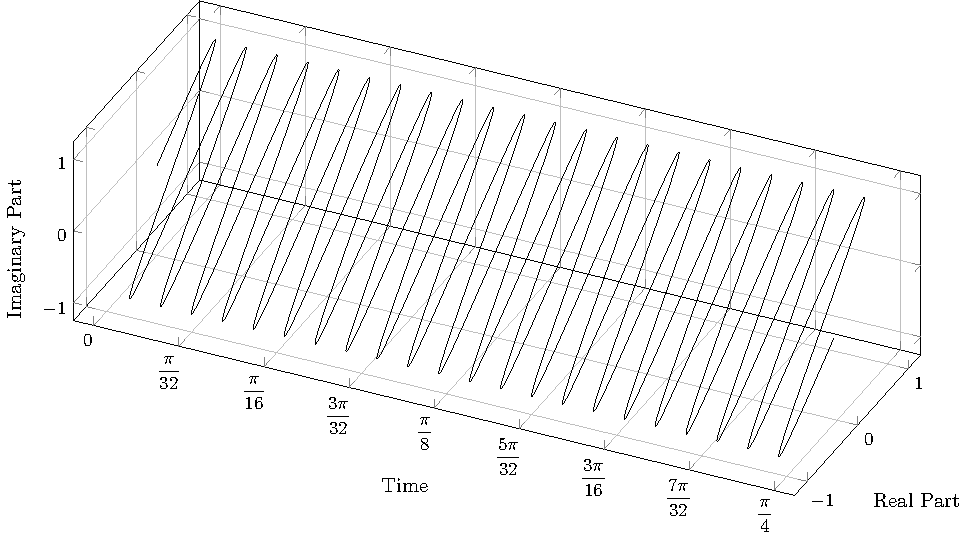
\includegraphics[height = \textheight] {tikzpics/plotComplexA.pdf}
            }
        }

        &
        \\

        \Block[c] {1-2} {
            \vbox{
                \captionof{figure} {3D view of \emph{complex sequence} A.}
                \label{plt:cmplxA}
            }
        }

        &
        \\

        \Block[c] {1-1} {
            \adjustbox{max width = \textwidth} {
                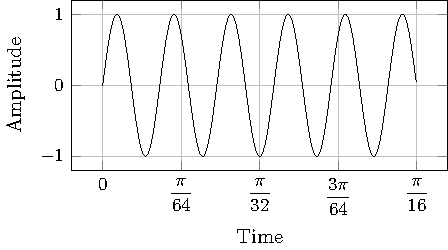
\includegraphics[height = \textheight] {tikzpics/plotShortX1.pdf}
            }
        }

        &

        \Block[c] {3-1} {
            \adjustbox{max width = \textwidth} {
                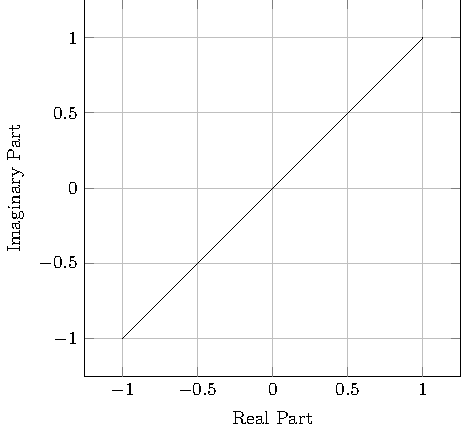
\includegraphics[height = \textheight] {tikzpics/plotFrontViewComplexA.pdf}
            }
        }

        \\

        \captionof{figure} {\emph{Real part} $\sin(2 \pi \freqXOne t)$.}
        \label{plt:realCmplxA}

        &
        \\

        \Block[c] {1-1} {
            \adjustbox{max width = \textwidth} {
                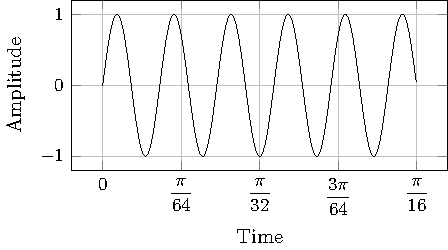
\includegraphics[height = \textheight] {tikzpics/plotShortX1.pdf}
            }
        }

        &
        \\

        \captionof{figure} {\emph{Imaginary part} $\sin(2 \pi \freqXOne t)$.}
        \label{plt:imagCmplxA}

        &

        \captionof{figure} {View with \emph{x axis} perpendicular.}
        \label{plt:frontViewCmplxA}

        \\

    \end{NiceTabularX}

\end{figure}


\subsection{Complex B} \label{ssec:visCplxB}
%% $x_{1} + j x_{2}$

\begin{itemize} [label=]

    \item \textbf{Sequence:} $\sin(2 \pi \freqXOne t) + j \sin(2 \pi \freqXTwo t)$

    \item \textbf{Inference:} Here the \emph{imaginary part} is higher in frequency than
        that of the \emph{real part}. This is similar to that of \textsc{Complex A} from
        Section \ref{ssec:visCplxA}, but this slight frequency difference will deviate the
        signal ever so slightly from oscillating through the straight line as viewed from
        the front view, and making the front view as shown in Figure \ref{plt:frontViewCmplxB}.

\end{itemize}

\vfill

\begin{figure} [H]

    \renewcommand{\arraystretch}{0.75}
    \centering
    \begin{NiceTabularX} {\textwidth} {
            *{2}{>{\centering\arraybackslash}X}
        }

        \Block[c] {1-2} {
            \adjustbox{max width = 2.0\textwidth} {
                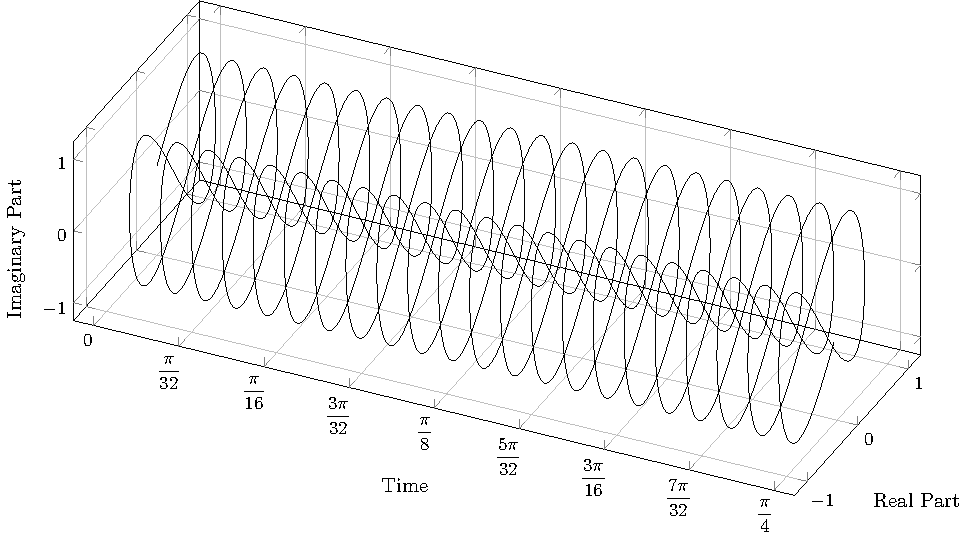
\includegraphics[height = \textheight] {tikzpics/plotComplexB.pdf}
            }
        }

        &
        \\

        \Block[c] {1-2} {
            \vbox{
                \captionof{figure} {3D view of \emph{complex sequence} B.}
                \label{plt:cmplxB}
            }
        }

        &
        \\

        \Block[c] {1-1} {
            \adjustbox{max width = \textwidth} {
                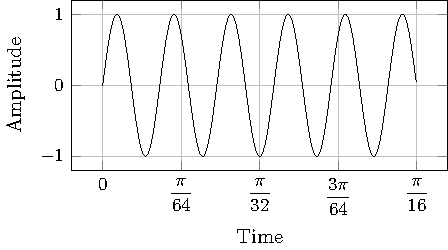
\includegraphics[height = \textheight] {tikzpics/plotShortX1.pdf}
            }
        }

        &

        \Block[c] {3-1} {
            \adjustbox{max width = \textwidth} {
                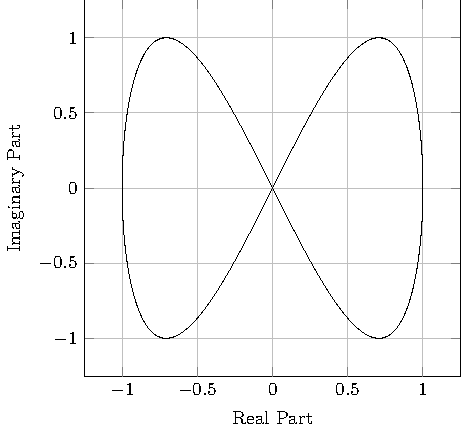
\includegraphics[height = \textheight] {tikzpics/plotFrontViewComplexB.pdf}
            }
        }

        \\

        \captionof{figure} {\emph{Real part} $\sin(2 \pi \freqXOne t)$.}
        \label{plt:realCmplxB}

        &
        \\

        \Block[c] {1-1} {
            \adjustbox{max width = \textwidth} {
                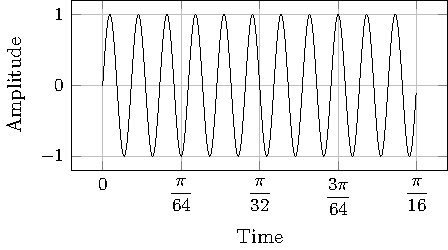
\includegraphics[height = \textheight] {tikzpics/plotShortX2.pdf}
            }
        }

        &
        \\

        \captionof{figure} {\emph{Imaginary part} $\sin(2 \pi \freqXTwo t)$.}
        \label{plt:imagCmplxB}

        &

        \captionof{figure} {View with \emph{x axis} perpendicular.}
        \label{plt:frontViewCmplxB}

        \\

    \end{NiceTabularX}

\end{figure}

\subsection{Complex C} \label{ssec:visCplxC}
%% $x_{1} + j x_{3}$

\begin{itemize} [label=]

    \item \textbf{Sequence:} $\sin(2 \pi \freqXOne t) + j \sin(2 \pi \freqXThree t)$

    \item \textbf{Inference:} Here the frequency of the \emph{imaginary part} is exactly the
        double that of the \emph{real part}. Hence forming an infinity\footnote{in mathematics, it's
        called a \emph{lemnicate} (see the \textbf{\href{https://en.m.wikipedia.org/wiki/Lemniscate_of_Bernoulli}
        {Wikipedia article}}).} shape from the front view.

\end{itemize}

\vfill

\begin{figure} [H]

    \renewcommand{\arraystretch}{0.75}
    \centering
    \begin{NiceTabularX} {\textwidth} {
            *{2}{>{\centering\arraybackslash}X}
        }

        \Block[c] {1-2} {
            \adjustbox{max width = 2.0\textwidth} {
                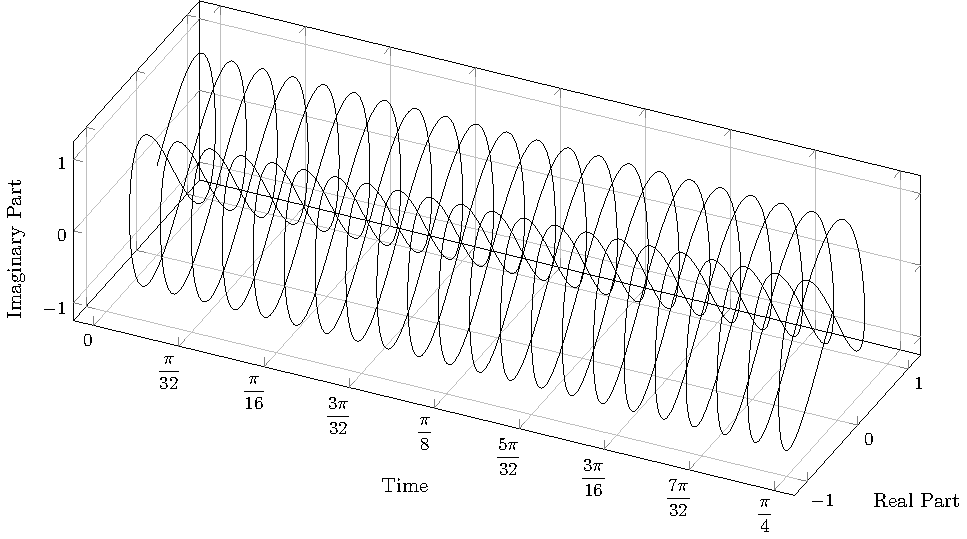
\includegraphics[height = \textheight] {tikzpics/plotComplexC.pdf}
            }
        }

        &
        \\

        \Block[c] {1-2} {
            \vbox{
                \captionof{figure} {3D view of \emph{complex sequence} C.}
                \label{plt:cmplxC}
            }
        }

        &
        \\

        \Block[c] {1-1} {
            \adjustbox{max width = \textwidth} {
                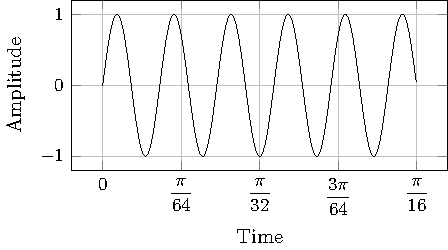
\includegraphics[height = \textheight] {tikzpics/plotShortX1.pdf}
            }
        }

        &

        \Block[c] {3-1} {
            \adjustbox{max width = \textwidth} {
                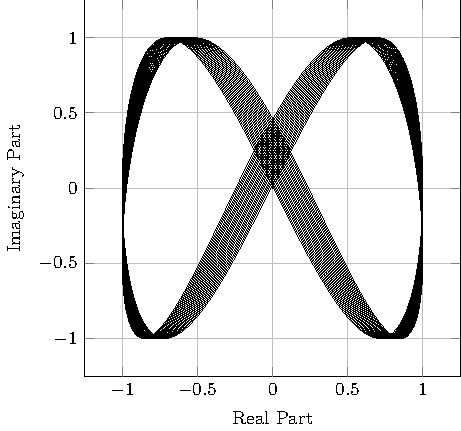
\includegraphics[height = \textheight] {tikzpics/plotFrontViewComplexC.pdf}
            }
        }

        \\

        \captionof{figure} {\emph{Real part} $\sin(2 \pi \freqXOne t)$.}
        \label{plt:realCmplxC}

        &
        \\

        \Block[c] {1-1} {
            \adjustbox{max width = \textwidth} {
                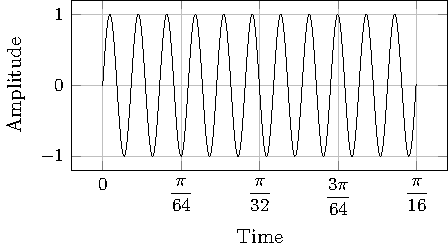
\includegraphics[height = \textheight] {tikzpics/plotShortX3.pdf}
            }
        }

        &
        \\

        \captionof{figure} {\emph{Imaginary part} $\sin(2 \pi \freqXThree t)$.}
        \label{plt:imagCmplxC}

        &

        \captionof{figure} {View with \emph{x axis} perpendicular.}
        \label{plt:frontViewCmplxC}

        \\

    \end{NiceTabularX}

\end{figure}

\subsection{Complex D} \label{ssec:visCplxD}
%% $x_{2} + j x_{1}$

\begin{itemize} [label=]

    \item \textbf{Sequence:} $\sin(2 \pi \freqXTwo t) + j \sin(2 \pi \freqXOne t)$

    \item \textbf{Inference:} This case is similar to \textsc{Complex B} from Section
        \ref{ssec:visCplxB}. The difference is the \emph{real} and \emph{imaginary} parts
        are swapped. And it results in the similar spiraling of the signal.

\end{itemize}

\vfill

\begin{figure} [H]

    \renewcommand{\arraystretch}{0.75}
    \centering
    \begin{NiceTabularX} {\textwidth} {
            *{2}{>{\centering\arraybackslash}X}
        }

        \Block[c] {1-2} {
            \adjustbox{max width = 2.0\textwidth} {
                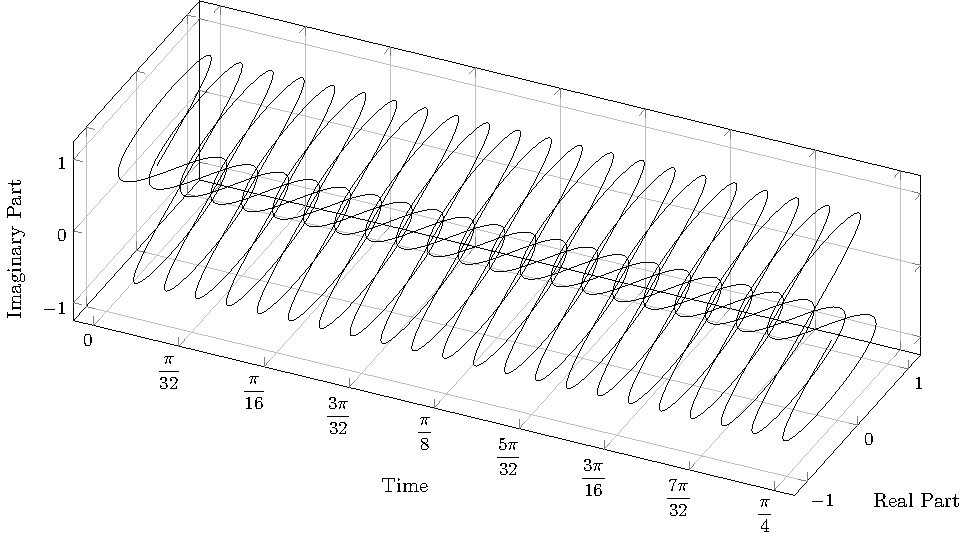
\includegraphics[height = \textheight] {tikzpics/plotComplexD.pdf}
            }
        }

        &
        \\

        \Block[c] {1-2} {
            \vbox{
                \captionof{figure} {3D view of \emph{complex sequence} D.}
                \label{plt:cmplxD}
            }
        }

        &
        \\

        \Block[c] {1-1} {
            \adjustbox{max width = \textwidth} {
                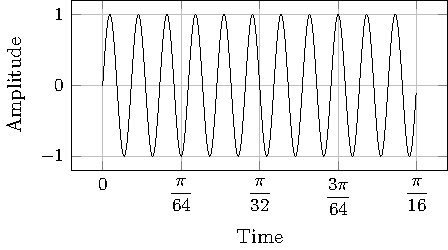
\includegraphics[height = \textheight] {tikzpics/plotShortX2.pdf}
            }
        }

        &

        \Block[c] {3-1} {
            \adjustbox{max width = \textwidth} {
                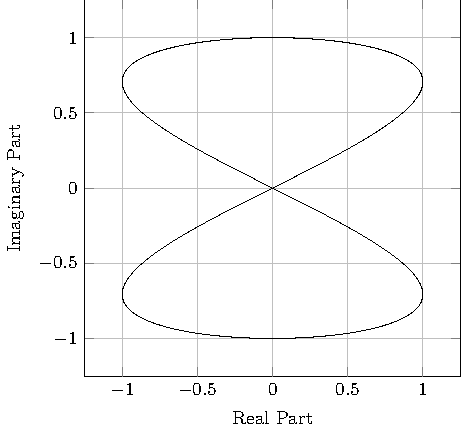
\includegraphics[height = \textheight] {tikzpics/plotFrontViewComplexD.pdf}
            }
        }

        \\

        \captionof{figure} {\emph{Real part} $\sin(2 \pi \freqXTwo t)$.}
        \label{plt:realCmplxD}

        &
        \\

        \Block[c] {1-1} {
            \adjustbox{max width = \textwidth} {
                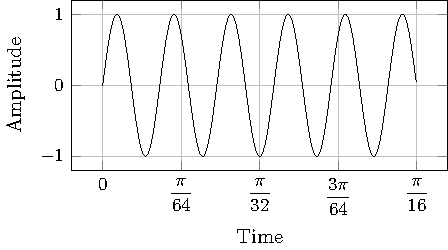
\includegraphics[height = \textheight] {tikzpics/plotShortX1.pdf}
            }
        }

        &
        \\

        \captionof{figure} {\emph{Imaginary part} $\sin(2 \pi \freqXOne t)$.}
        \label{plt:imagCmplxD}

        &

        \captionof{figure} {View with \emph{x axis} perpendicular.}
        \label{plt:frontViewCmplxD}

        \\

    \end{NiceTabularX}

\end{figure}

\subsection{Complex E} \label{ssec:visCplxE}
%% $x_{2} + j x_{2}$

\begin{itemize} [label=]

    \item \textbf{Sequence:} $\sin(2 \pi \freqXTwo t) + j \sin(2 \pi \freqXTwo t)$

    \item \textbf{Inference:} This is similar to that of \textsc{Complex A} from Section
        \ref{ssec:visCplxA}, here both the \emph{real} and \emph{imaginary} parts are the
        same. Hence, causing an oscillation through a straight line.

\end{itemize}

\vfill

\begin{figure} [H]

    \renewcommand{\arraystretch}{0.75}
    \centering
    \begin{NiceTabularX} {\textwidth} {
            *{2}{>{\centering\arraybackslash}X}
        }

        \Block[c] {1-2} {
            \adjustbox{max width = 2.0\textwidth} {
                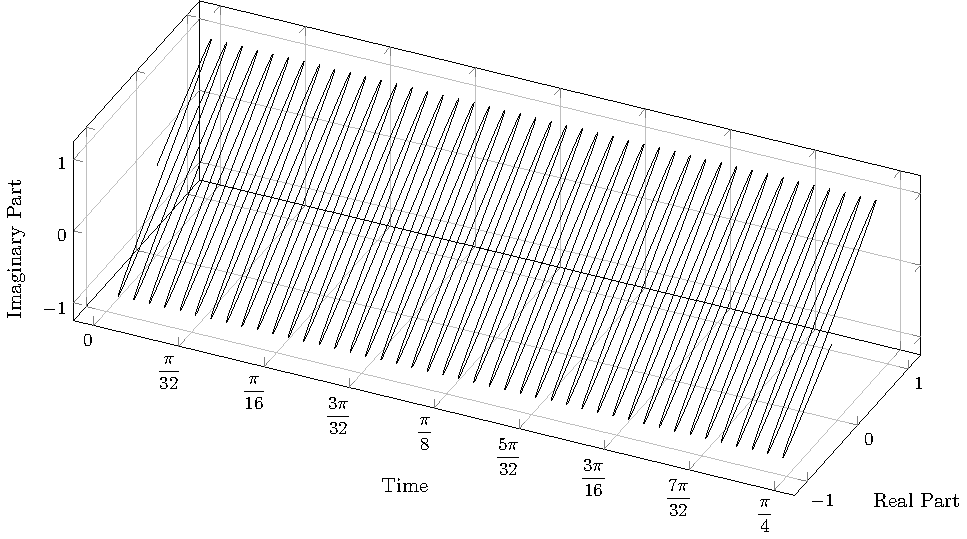
\includegraphics[height = \textheight] {tikzpics/plotComplexE.pdf}
            }
        }

        &
        \\

        \Block[c] {1-2} {
            \vbox{
                \captionof{figure} {3D view of \emph{complex sequence} E.}
                \label{plt:cmplxE}
            }
        }

        &
        \\

        \Block[c] {1-1} {
            \adjustbox{max width = \textwidth} {
                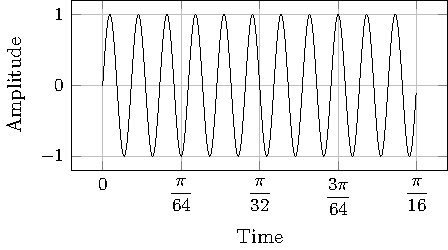
\includegraphics[height = \textheight] {tikzpics/plotShortX2.pdf}
            }
        }

        &

        \Block[c] {3-1} {
            \adjustbox{max width = \textwidth} {
                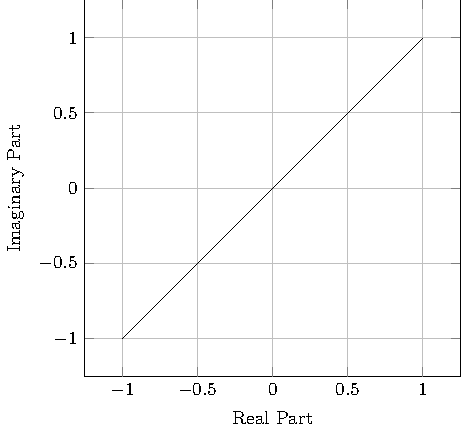
\includegraphics[height = \textheight] {tikzpics/plotFrontViewComplexE.pdf}
            }
        }

        \\

        \captionof{figure} {\emph{Real part} $\sin(2 \pi \freqXTwo t)$.}
        \label{plt:realCmplxE}

        &
        \\

        \Block[c] {1-1} {
            \adjustbox{max width = \textwidth} {
                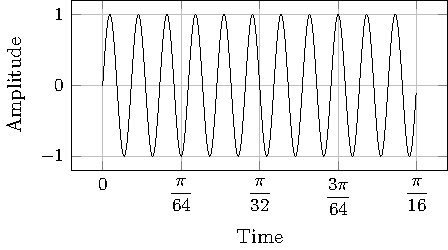
\includegraphics[height = \textheight] {tikzpics/plotShortX2.pdf}
            }
        }

        &
        \\

        \captionof{figure} {\emph{Imaginary part} $\sin(2 \pi \freqXTwo t)$.}
        \label{plt:imagCmplxE}

        &

        \captionof{figure} {View with \emph{x axis} perpendicular.}
        \label{plt:frontViewCmplxE}

        \\

    \end{NiceTabularX}

\end{figure}

\subsection{Complex F} \label{ssec:visCplxF}
%% $x_{2} + j x_{3}$

\begin{itemize} [label=]

    \item \textbf{Sequence:} $\sin(2 \pi \freqXTwo t) + j \sin(2 \pi \freqXThree t)$

    \item \textbf{Inference:} Here the \emph{real} and \emph{imaginary} parts are similar
        to that of \textsc{Complex C} from Section \ref{ssec:visCplxC}. The only difference
        is that the \emph{frequency} of the \emph{imaginary part} is not exactly the double
        that of the \emph{real part}. This causes the signal to deviate from that infinity shape.
        This becomes evident as we observe the front view from the Figure \ref{plt:frontViewCmplxF}.

\end{itemize}

\vfill

\begin{figure} [H]

    \renewcommand{\arraystretch}{0.75}
    \centering
    \begin{NiceTabularX} {\textwidth} {
            *{2}{>{\centering\arraybackslash}X}
        }

        \Block[c] {1-2} {
            \adjustbox{max width = 2.0\textwidth} {
                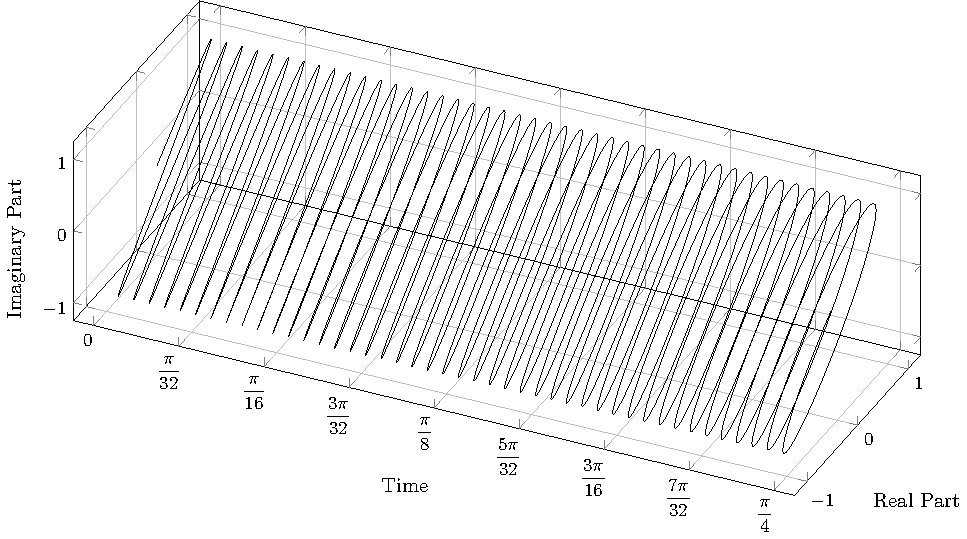
\includegraphics[height = \textheight] {tikzpics/plotComplexF.pdf}
            }
        }

        &
        \\

        \Block[c] {1-2} {
            \vbox{
                \captionof{figure} {3D view of \emph{complex sequence} F.}
                \label{plt:cmplxF}
            }
        }

        &
        \\

        \Block[c] {1-1} {
            \adjustbox{max width = \textwidth} {
                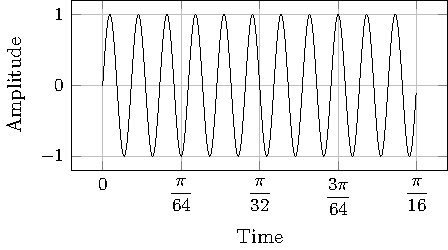
\includegraphics[height = \textheight] {tikzpics/plotShortX2.pdf}
            }
        }

        &

        \Block[c] {3-1} {
            \adjustbox{max width = \textwidth} {
                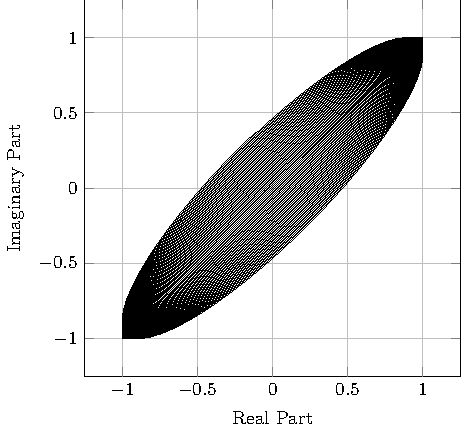
\includegraphics[height = \textheight] {tikzpics/plotFrontViewComplexF.pdf}
            }
        }

        \\

        \captionof{figure} {\emph{Real part} $\sin(2 \pi \freqXTwo t)$.}
        \label{plt:realCmplxF}

        &
        \\

        \Block[c] {1-1} {
            \adjustbox{max width = \textwidth} {
                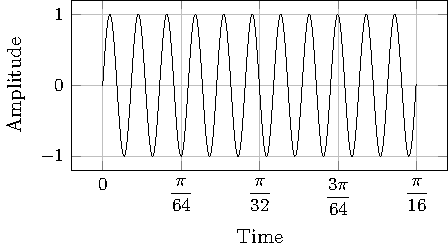
\includegraphics[height = \textheight] {tikzpics/plotShortX3.pdf}
            }
        }

        &
        \\

        \captionof{figure} {\emph{Imaginary part} $\sin(2 \pi \freqXThree t)$.}
        \label{plt:imagCmplxF}

        &

        \captionof{figure} {View with \emph{x axis} perpendicular.}
        \label{plt:frontViewCmplxF}

        \\

    \end{NiceTabularX}

\end{figure}

\subsection{Complex G} \label{ssec:visCplxG}
%% $x_{3} + j x_{1}$

\begin{itemize} [label=]

    \item \textbf{Sequence:} $\sin(2 \pi \freqXThree t) + j \sin(2 \pi \freqXOne t)$

    \item \textbf{Inference:} This is similar to \textsc{Complex C} from Section \ref{ssec:visCplxC}.
        The only difference is that the \emph{real part} and the \emph{imaginary part} are swapped.

\end{itemize}

\vfill

\begin{figure} [H]

    \renewcommand{\arraystretch}{0.75}
    \centering
    \begin{NiceTabularX} {\textwidth} {
            *{2}{>{\centering\arraybackslash}X}
        }

        \Block[c] {1-2} {
            \adjustbox{max width = 2.0\textwidth} {
                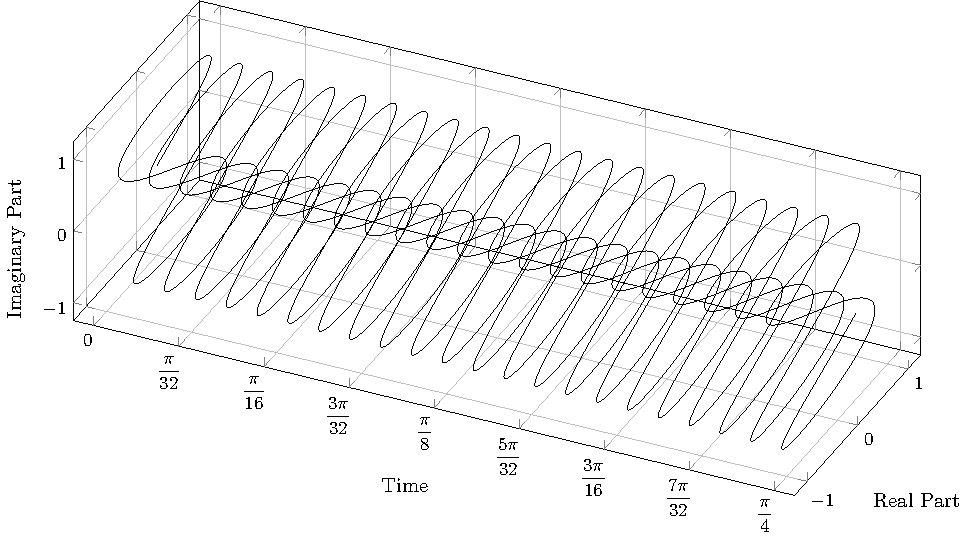
\includegraphics[height = \textheight] {tikzpics/plotComplexG.pdf}
            }
        }

        &
        \\

        \Block[c] {1-2} {
            \vbox{
                \captionof{figure} {3D view of \emph{complex sequence} G.}
                \label{plt:cmplxG}
            }
        }

        &
        \\

        \Block[c] {1-1} {
            \adjustbox{max width = \textwidth} {
                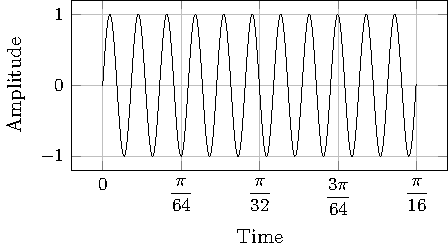
\includegraphics[height = \textheight] {tikzpics/plotShortX3.pdf}
            }
        }

        &

        \Block[c] {3-1} {
            \adjustbox{max width = \textwidth} {
                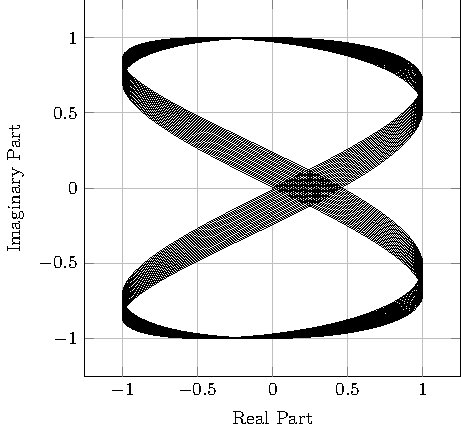
\includegraphics[height = \textheight] {tikzpics/plotFrontViewComplexG.pdf}
            }
        }

        \\

        \captionof{figure} {\emph{Real part} $\sin(2 \pi \freqXThree t)$.}
        \label{plt:realCmplxG}

        &
        \\

        \Block[c] {1-1} {
            \adjustbox{max width = \textwidth} {
                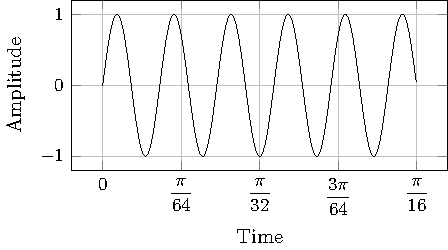
\includegraphics[height = \textheight] {tikzpics/plotShortX1.pdf}
            }
        }

        &
        \\

        \captionof{figure} {\emph{Imaginary part} $\sin(2 \pi \freqXOne t)$.}
        \label{plt:imagCmplxG}

        &

        \captionof{figure} {View with \emph{x axis} perpendicular.}
        \label{plt:frontViewCmplxG}

        \\

    \end{NiceTabularX}

\end{figure}

\subsection{Complex H} \label{ssec:visCplxH}
%% $x_{3} + j x_{2}$

\begin{itemize} [label=]

    \item \textbf{Sequence:} $\sin(2 \pi \freqXThree t) + j \sin(2 \pi \freqXTwo t)$

    \item \textbf{Inference:} This case is similar that of \textsc{Complex F} from Section
        \ref{ssec:visCplxF}. The difference is that the \emph{real} and the \emph{imaginary}
        parts are swapped.

\end{itemize}

\vfill

\begin{figure} [H]

    \renewcommand{\arraystretch}{0.75}
    \centering
    \begin{NiceTabularX} {\textwidth} {
            *{2}{>{\centering\arraybackslash}X}
        }

        \Block[c] {1-2} {
            \adjustbox{max width = 2.0\textwidth} {
                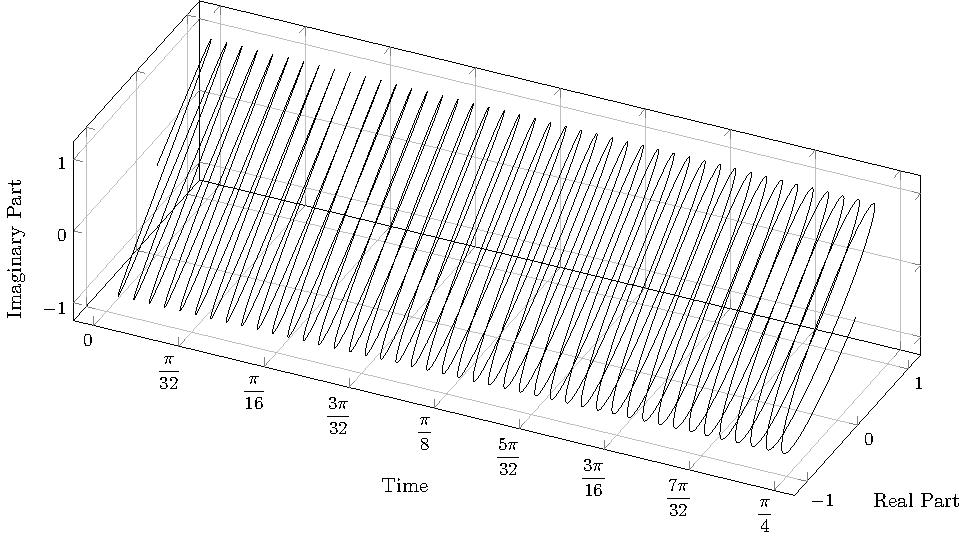
\includegraphics[height = \textheight] {tikzpics/plotComplexH.pdf}
            }
        }

        &
        \\

        \Block[c] {1-2} {
            \vbox{
                \captionof{figure} {3D view of \emph{complex sequence} H.}
                \label{plt:cmplxH}
            }
        }

        &
        \\

        \Block[c] {1-1} {
            \adjustbox{max width = \textwidth} {
                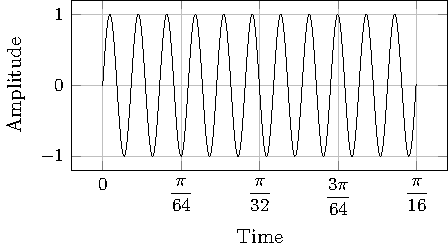
\includegraphics[height = \textheight] {tikzpics/plotShortX3.pdf}
            }
        }

        &

        \Block[c] {3-1} {
            \adjustbox{max width = \textwidth} {
                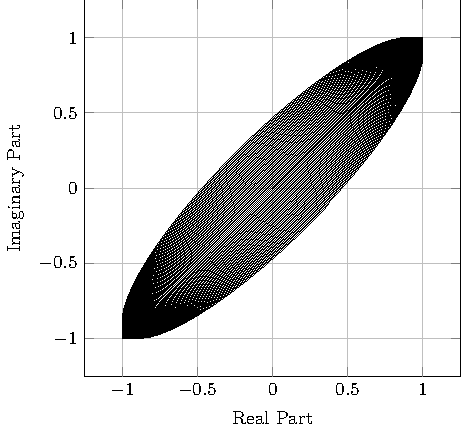
\includegraphics[height = \textheight] {tikzpics/plotFrontViewComplexH.pdf}
            }
        }

        \\

        \captionof{figure} {\emph{Real part} $\sin(2 \pi \freqXThree t)$.}
        \label{plt:realCmplxH}

        &
        \\

        \Block[c] {1-1} {
            \adjustbox{max width = \textwidth} {
                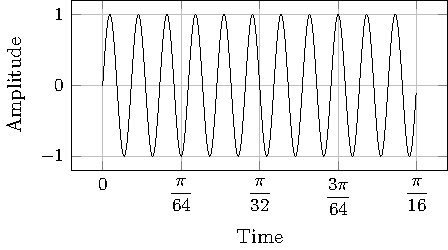
\includegraphics[height = \textheight] {tikzpics/plotShortX2.pdf}
            }
        }

        &
        \\

        \captionof{figure} {\emph{Imaginary part} $\sin(2 \pi \freqXTwo t)$.}
        \label{plt:imagCmplxH}

        &

        \captionof{figure} {View with \emph{x axis} perpendicular.}
        \label{plt:frontViewCmplxH}

        \\

    \end{NiceTabularX}

\end{figure}

\subsection{Complex I} \label{ssec:visCplxI}
%% $x_{3} + j x_{3}$

\begin{itemize} [label=]

    \item \textbf{Sequence:} $\sin(2 \pi \freqXThree t) + j \sin(2 \pi \freqXThree t)$

    \item \textbf{Inference:} This case is similar to that of \textsc{Complex A} and
        \textsc{Complex E} from Sections \ref{ssec:visCplxA} and \ref{ssec:visCplxE}
        respectively. Both the \emph{real} and \emph{imaginary} parts are the same,
        hence the front view is a straight line as seen in Figure \ref{plt:frontViewCmplxI}.

\end{itemize}

\vfill

\begin{figure} [H]

    \renewcommand{\arraystretch}{0.75}
    \centering
    \begin{NiceTabularX} {\textwidth} {
            *{2}{>{\centering\arraybackslash}X}
        }

        \Block[c] {1-2} {
            \adjustbox{max width = 2.0\textwidth} {
                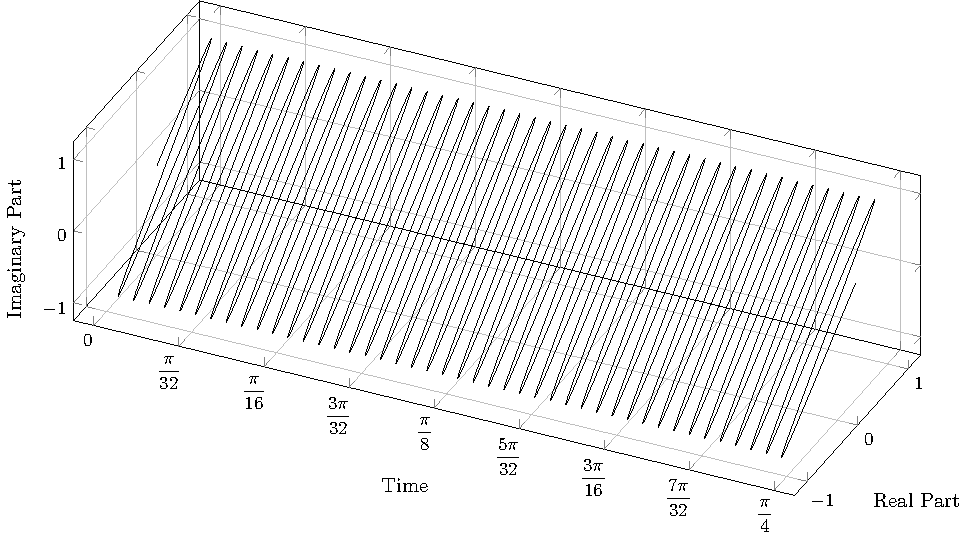
\includegraphics[height = \textheight] {tikzpics/plotComplexI.pdf}
            }
        }

        &
        \\

        \Block[c] {1-2} {
            \vbox{
                \captionof{figure} {3D view of \emph{complex sequence} I.}
                \label{plt:cmplxI}
            }
        }

        &
        \\

        \Block[c] {1-1} {
            \adjustbox{max width = \textwidth} {
                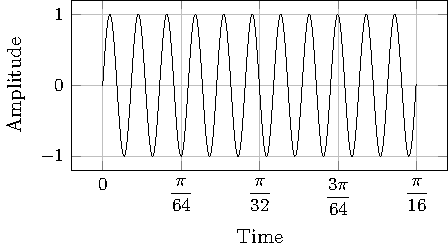
\includegraphics[height = \textheight] {tikzpics/plotShortX3.pdf}
            }
        }

        &

        \Block[c] {3-1} {
            \adjustbox{max width = \textwidth} {
                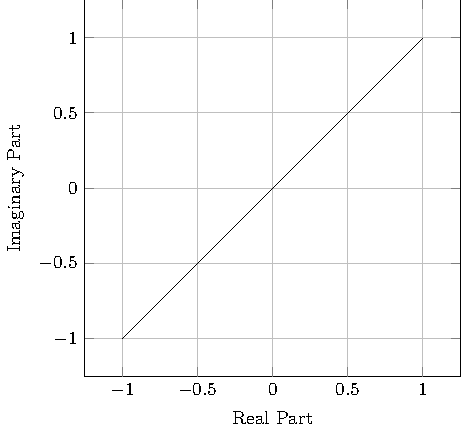
\includegraphics[height = \textheight] {tikzpics/plotFrontViewComplexI.pdf}
            }
        }

        \\

        \captionof{figure} {\emph{Real part} $\sin(2 \pi \freqXThree t)$.}
        \label{plt:realCmplxI}

        &
        \\

        \Block[c] {1-1} {
            \adjustbox{max width = \textwidth} {
                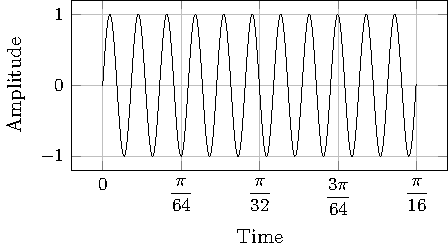
\includegraphics[height = \textheight] {tikzpics/plotShortX3.pdf}
            }
        }

        &
        \\

        \captionof{figure} {\emph{Imaginary part} $\sin(2 \pi \freqXThree t)$.}
        \label{plt:imagCmplxI}

        &

        \captionof{figure} {View with \emph{x axis} perpendicular.}
        \label{plt:frontViewCmplxI}

        \\

    \end{NiceTabularX}

\end{figure}



%% \begin{figure}
%%     \centering
%%     \adjustbox{max width = \textwidth} {
%%         \includegraphics[height = 0.8\textheight] {tikzpics/testing.pdf}
%%     }
%%     \captionof{figure} {Testing}
%%     \label{plt:testing}
%% \end{figure}
%%
%%
%% \begin{figure}
%%     \centering
%%     \adjustbox{max width = 0.7\textwidth} {
%%         \includegraphics[height = 0.8\textheight] {tikzpics/hai.pdf}
%%     }
%%     \captionof{figure} {Ahai}
%%     \label{plt:wowo}
%% \end{figure}
%%
%%
%%
%% \begin{figure}
%%     \centering
%%     \adjustbox{max width = 0.7\textwidth} {
%%         \includegraphics[height = 0.8\textheight] {tikzpics/woo.pdf}
%%     }
%%     \captionof{figure} {Ahai}
%%     \label{plt:wowo}
%% \end{figure}





\end{document}
